\documentclass[11pt,border=6pt]{standalone}
\usepackage{fontspec}
\usepackage{tikz}
\usetikzlibrary{positioning,arrows.meta,calc,fit,backgrounds}
\begin{document}
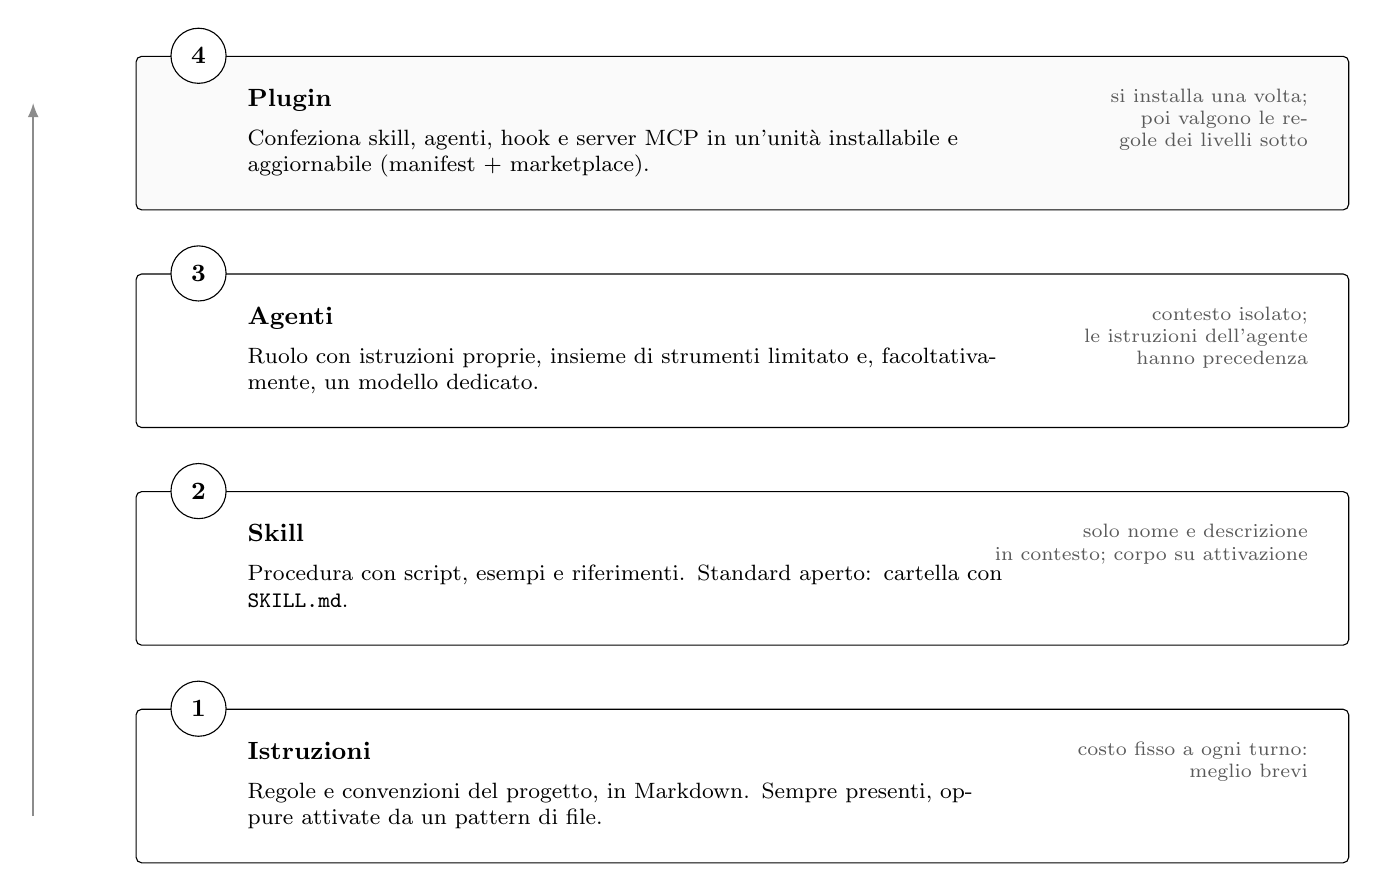
\begin{tikzpicture}[font=\footnotesize,
  lvl/.style={draw, rounded corners=2pt, minimum width=15.4cm, minimum height=1.95cm,
    align=left, inner sep=5pt},
  num/.style={circle, draw, minimum size=7mm, inner sep=0pt, font=\small\bfseries},
  ttl/.style={font=\small\bfseries},
  note/.style={font=\scriptsize, text=black!65},
  arr/.style={-{Latex[length=1.8mm,width=1.4mm]}, black!45, semithick}]

  % Livello 4 — plugin
  \node[lvl, fill=black!2] (l4) at (0,0) {};
  \node[num, fill=white] at ([xshift=8mm]l4.north west) {4};
  \node[ttl, anchor=north west] at ([xshift=13mm,yshift=-3mm]l4.north west) {Plugin};
  \node[anchor=north west, align=left, text width=9.6cm] at ([xshift=13mm,yshift=-8.2mm]l4.north west)
    {Confeziona skill, agenti, hook e server MCP in un'unità installabile e aggiornabile (manifest + marketplace).};
  \node[note, anchor=north east, align=right, text width=4.4cm] at ([xshift=-4mm,yshift=-3mm]l4.north east)
    {si installa una volta;\\poi valgono le regole dei livelli sotto};

  % Livello 3 — agenti
  \node[lvl, below=8mm of l4] (l3) {};
  \node[num, fill=white] at ([xshift=8mm]l3.north west) {3};
  \node[ttl, anchor=north west] at ([xshift=13mm,yshift=-3mm]l3.north west) {Agenti};
  \node[anchor=north west, align=left, text width=9.6cm] at ([xshift=13mm,yshift=-8.2mm]l3.north west)
    {Ruolo con istruzioni proprie, insieme di strumenti limitato e, facoltativamente, un modello dedicato.};
  \node[note, anchor=north east, align=right, text width=4.4cm] at ([xshift=-4mm,yshift=-3mm]l3.north east)
    {contesto isolato;\\le istruzioni dell'agente\\hanno precedenza};

  % Livello 2 — skill
  \node[lvl, below=8mm of l3] (l2) {};
  \node[num, fill=white] at ([xshift=8mm]l2.north west) {2};
  \node[ttl, anchor=north west] at ([xshift=13mm,yshift=-3mm]l2.north west) {Skill};
  \node[anchor=north west, align=left, text width=9.6cm] at ([xshift=13mm,yshift=-8.2mm]l2.north west)
    {Procedura con script, esempi e riferimenti. Standard aperto: cartella con \texttt{SKILL.md}.};
  \node[note, anchor=north east, align=right, text width=4.4cm] at ([xshift=-4mm,yshift=-3mm]l2.north east)
    {solo nome e descrizione\\in contesto; corpo su attivazione};

  % Livello 1 — istruzioni
  \node[lvl, below=8mm of l2] (l1) {};
  \node[num, fill=white] at ([xshift=8mm]l1.north west) {1};
  \node[ttl, anchor=north west] at ([xshift=13mm,yshift=-3mm]l1.north west) {Istruzioni};
  \node[anchor=north west, align=left, text width=9.6cm] at ([xshift=13mm,yshift=-8.2mm]l1.north west)
    {Regole e convenzioni del progetto, in Markdown. Sempre presenti, oppure attivate da un pattern di file.};
  \node[note, anchor=north east, align=right, text width=4.4cm] at ([xshift=-4mm,yshift=-3mm]l1.north east)
    {costo fisso a ogni turno:\\meglio brevi};

  % asse del costo
  \draw[arr] ([xshift=-13mm,yshift=6mm]l1.south west) -- ([xshift=-13mm,yshift=-6mm]l4.north west);
\end{tikzpicture}
\end{document}
